% sample.tex
\documentclass[pdf,swa,slideBW,nocolorBG,nototal]{prosper}
%\usepackage{ngerman}
\usepackage{graphicx}
\usepackage{wrapfig, rotating}
\usepackage[T1]{fontenc}

\title{Tracing Object Lifetime}
\author{Christoph Neijenhuis, Tobias Mohr, Tim Felgentreff}
%\email{\{christoph.neijenhuis, tobias.mohr, fim.felgentreff\}@student.hpi.uni-potsdam.de}
\institution{
        Agile Software Development \\
        Hasso-Plattner-Institut \\
        Universit�t Potsdam\\
        SS 2011
}
\foot{Agile Software Development 2011 | Felgentreff, Mohr, Neijenhuis | \today }

\begin{document}

\maketitle

\begin{slide}{Demo}
  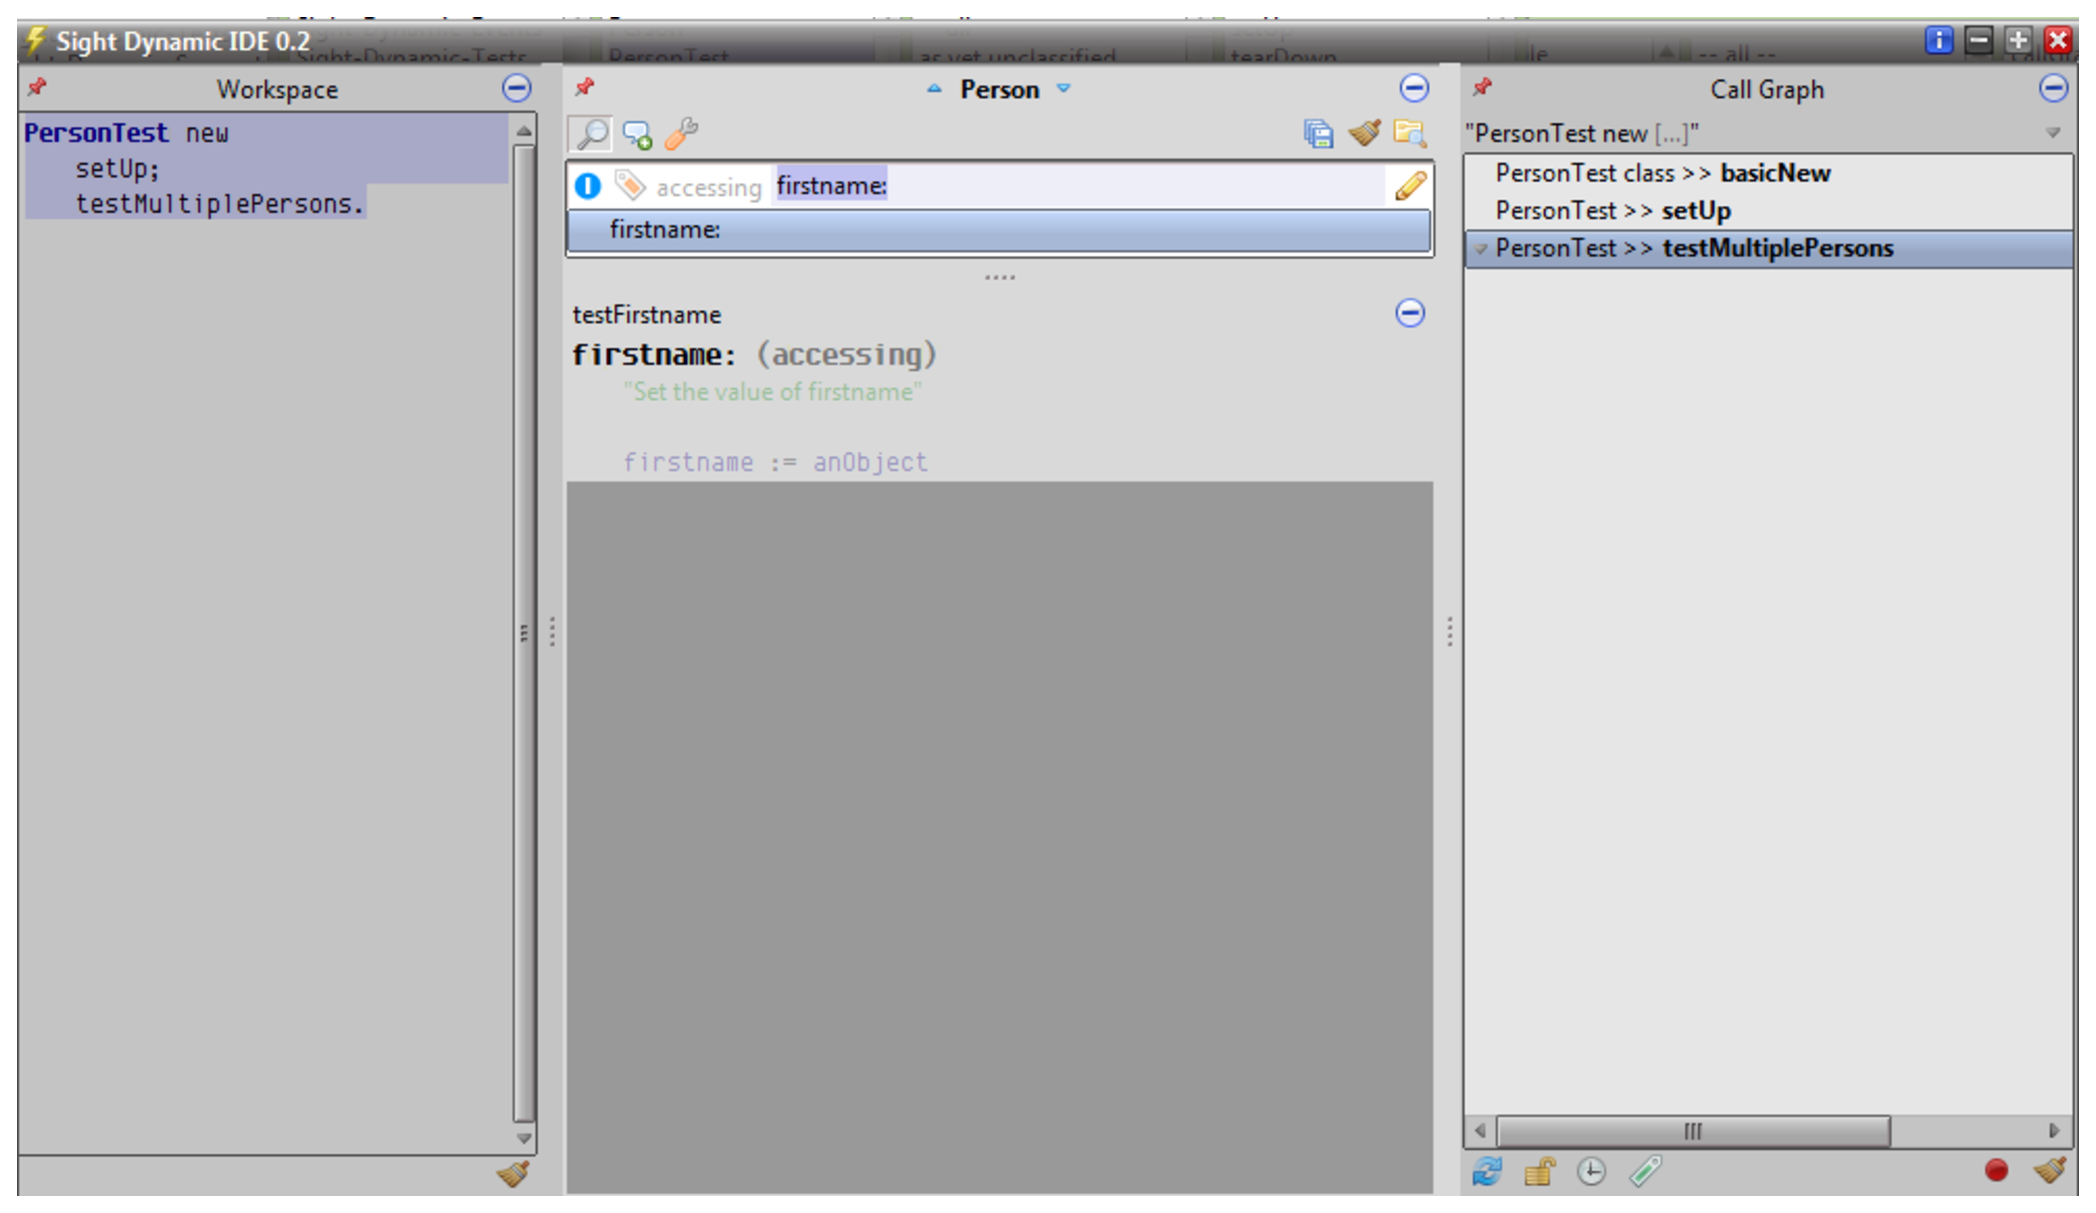
\includegraphics[width=\linewidth]{pics/sdide_intro}
\end{slide}

% \overlays{2}{%
% \begin{slide}{Demo}
%   \begin{itemize}
%   \item During its lifetime an object is \ldots
%     \begin{itemize}
%     \item created from a class,
%     \item referenced in different contexts,
%     \item called upon,
%     \item and modified.
%     \end{itemize}
%   \end{itemize}
%   \fromSlide{2}{%
%   \begin{itemize}
%     \item The call graph tracer is a way to ask questions
%     \begin{itemize}
%     \item Where did this object come from?
%     \item Who calls it and when?
%     \item Where and how is it modified?
%     \item How does it arrive at a particular point?
%     \end{itemize}
%   \end{itemize}}
% \end{slide}}

\begin{slide}{Agenda}
  \begin{itemize}
  \item Come again (Previously, on Agile-SD-1)
  \item Developer Stories (A New Scope)
  \item Different Visions (Research Strikes Back)
  \item Improved Tests (Return of Readability)
  \end{itemize}
\end{slide}

\overlays{2}{%
\begin{slide}{Previously\ldots}
  \begin{itemize}
  \item Management with ``offline'' story cards
  \item Bi-weekly meetings
  \item Weekly story choices \& estimates
  \end{itemize}
  \fromSlide{2}{%
    {\bf Critique}
    \begin{itemize}
    \item Insufficient traceability
    \item Somewhat fragile testing \& continuous testing infrastructure
    \item General lack of motivating vision
    \end{itemize}}
\end{slide}
}

% \overlays{4}{%
% \begin{slide}{Tests}
%   \begin{itemize}
%   \item Tests were developed in parallel to the implementation
%     \fromSlide{2}{%
%       \begin{itemize}
%       \item As a quicker workspace
%       \item To run examples quickly
%       \fromSlide{3}{%
%       \item \ldots, but not to test user stories}
%     \end{itemize}}
%   \fromSlide{4}{%
%   \item $\Rightarrow$ It's hard to write tests in the beginning}
%   \end{itemize}
% \end{slide}}

% \begin{slide}{Tests}
%   \begin{minipage}{0.6\linewidth}
%     \begin{centering}
%       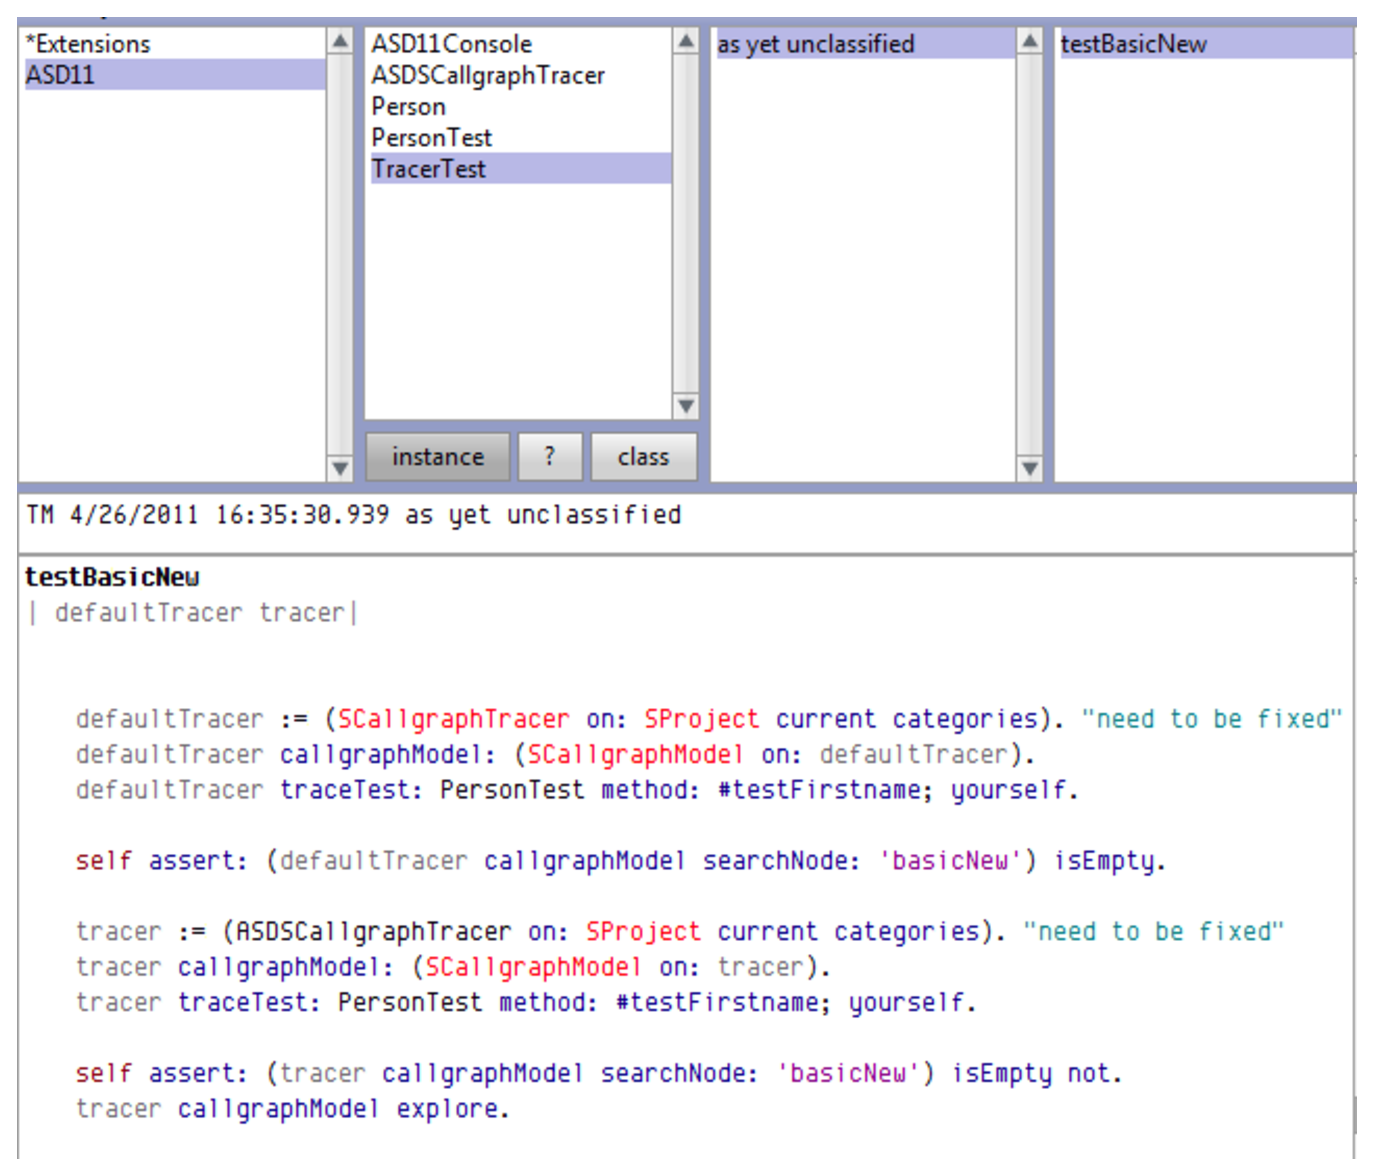
\includegraphics[width=\linewidth]{pics/workspace_test}
%     \end{centering}
%   \end{minipage}
%   \begin{minipage}{0.3\linewidth}
%     \raggedright{Note the {\bf \#explore} at the bottom}
%   \end{minipage}
% \end{slide}

% \overlays{3}{%
% \begin{slide}{Problems with testing}
%   \begin{itemize}
%   \item Criticism from the customer after first sprint
%   \fromSlide{2}{%
%     \begin{itemize}
%     \item Tests are hard to understand
%     \item Tests are not easily matched to user stories
%     \end{itemize}
%   }
%   \end{itemize}
%   \fromSlide{3}{%
%     \raggedleft{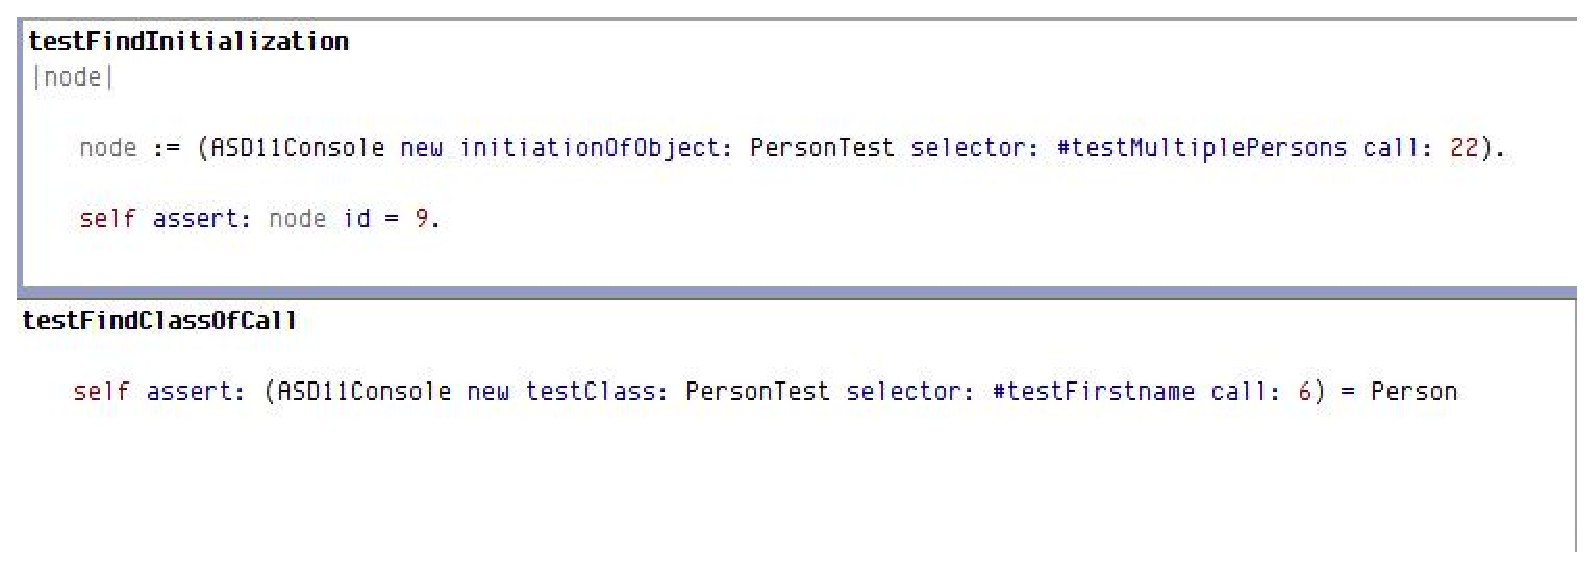
\includegraphics[width=0.8\linewidth]{pics/bad_tests}}
%   }
% \end{slide}}

% \overlays{2}{%
% \begin{slide}{Problems with testing}
%   \begin{itemize}
%   \item For the second sprint we started with implementing the tests
%     first, \ldots
%     \begin{itemize}
%     \item \ldots but then decided to re-implement based on different code.
%     \end{itemize}
%   \fromSlide{2}{%
%   \item At the end of Sprint \#2, we don't have tests for all functionality}
%   \end{itemize}
% \end{slide}}

% \begin{slide}{Conclusions}
%   \begin{itemize}
%   \item We're doing well estimating overall time
%     \begin{itemize}
%     \item The first sprint we managed to implement all, the second
%       half the stories
%     \item Our estimates were off on the work required to acquaint
%       ourselves with the framework
%     \item Tickets, as well as stories, would be nice to track that
%       ``additional work''
%     \end{itemize}
%   \item We need to track our time per story more closely to get better
%     on that granularity, too
%   \item We have to be more stringent with {\bf ``test first''}
%   \item We need tests to begin with
%   \end{itemize}
% \end{slide}

\begin{slide}{}
  \nocite{*}
  \bibliographystyle{splncs}
  {\small \bibliography{swt.bib}}
\end{slide}

\end{document}
